% Chapter 4

\chapter{Experiments} % Main chapter title

\label{Chapter4} % For referencing the chapter elsewhere, use \ref{Chapter1} 

\lhead{Chapter 4. \emph{Experiments}} % This is for the header on each page - perhaps a shortened title

This chapter describes the experiments carried out to evaluate the proposed solution. 
 
\section{Description of the dataset} \label{4.1}

The data provided for the evaluation of the system comes from another experiment developed in the Department of Automation and Systems Engineering at Universidad Carlos III de Madrid in the field of gesture and pose recognition \cite{Gonzalez-Pacheco2013}. It consisted of 24 users who taught the robot a predetermined set of poses using a Microsoft Kinect camera, the data retrieved was then labeled by the user trough a voice interaction with the user. Figure \ref{fig:scen} shows the disposition of the experiment. It consisted of a Kinect camera placed inside the Social Robot Maggie \cite{maggie}, in the figure the cone represents the field of view of the Kinect sensor. The user was allowed to move inside the rectangle.

\begin{figure}[h]
\includegraphics[width=7cm]{Figures/Scenario}
\centering
\caption{Scenario of the experiment. Retrieved from \cite{Gonzalez-Pacheco2013}. \label{fig:scen}}
\end{figure}

The data retrieved from the user is a set of parameters that represent the 3D position of 15 joints of a human skeleton. The disposition of the data is showed in Figure \ref{fig:kine}. The entries of the dataset have the following shape:

\begin{figure}[h]
\includegraphics[width=8cm]{Figures/Skeleton}
\centering
\caption{Kinematic of the human body. Retrieved from \cite{Gonzalez-Pacheco2013}- \label{fig:kine}}
\end{figure}
 
Each instance I is a set of $t$ the time stamp sequence number, $u$ the user ID, $J$ the set of joints and $L$ the label of the entry.\label{eq-4.1}
\begin{equation} 
I = (t,u,J,L)
\end{equation}
Each set of joints is formed by 15 joints, that can be seen in Figure \ref{fig:kine}.\label{eq-4.2}
\begin{equation} 
J = (j_1,j_2,...,j_15) 
\end{equation}
Each of the joints is formed by x,y,z 3D positions, qx,qy,qz,qw, orientations and a confidence C.\label{eq-4.3}
\begin{equation} 
j_i = (x,y,z,qx,qy,qz,qw,C) 
\end{equation}

The experiment was subdivided in 3 sets of poses taught to the robot:

\begin{description}
\item[Set 1] consisted in teaching the robot if the trainer was turned to his/her own left, right or if he/she was turned toward the robot.
\item[Set 2] consisted in teaching the robot if the trainer was looking to his/her own left, right or forward.
\item[Set 3]consisted in teaching the robot if the trainer was pointing at his/her own left, right or forward. Example shown in Figure \ref{fig:set3}.
\end{description}

\section{Data treatment for this experiment} \label{4.2}

The data used for this Thesis was extracted from Set 3 of the experiment mentioned in Section \ref{4.1}, where users pointed right, left and forward. In Figure \ref{fig:set3}, picture (a) is an example of a user pointing \emph{left}, in (b) the user is pointing \emph{forward} and in (c) the user is pointing \emph{right}.

\begin{figure}[h]
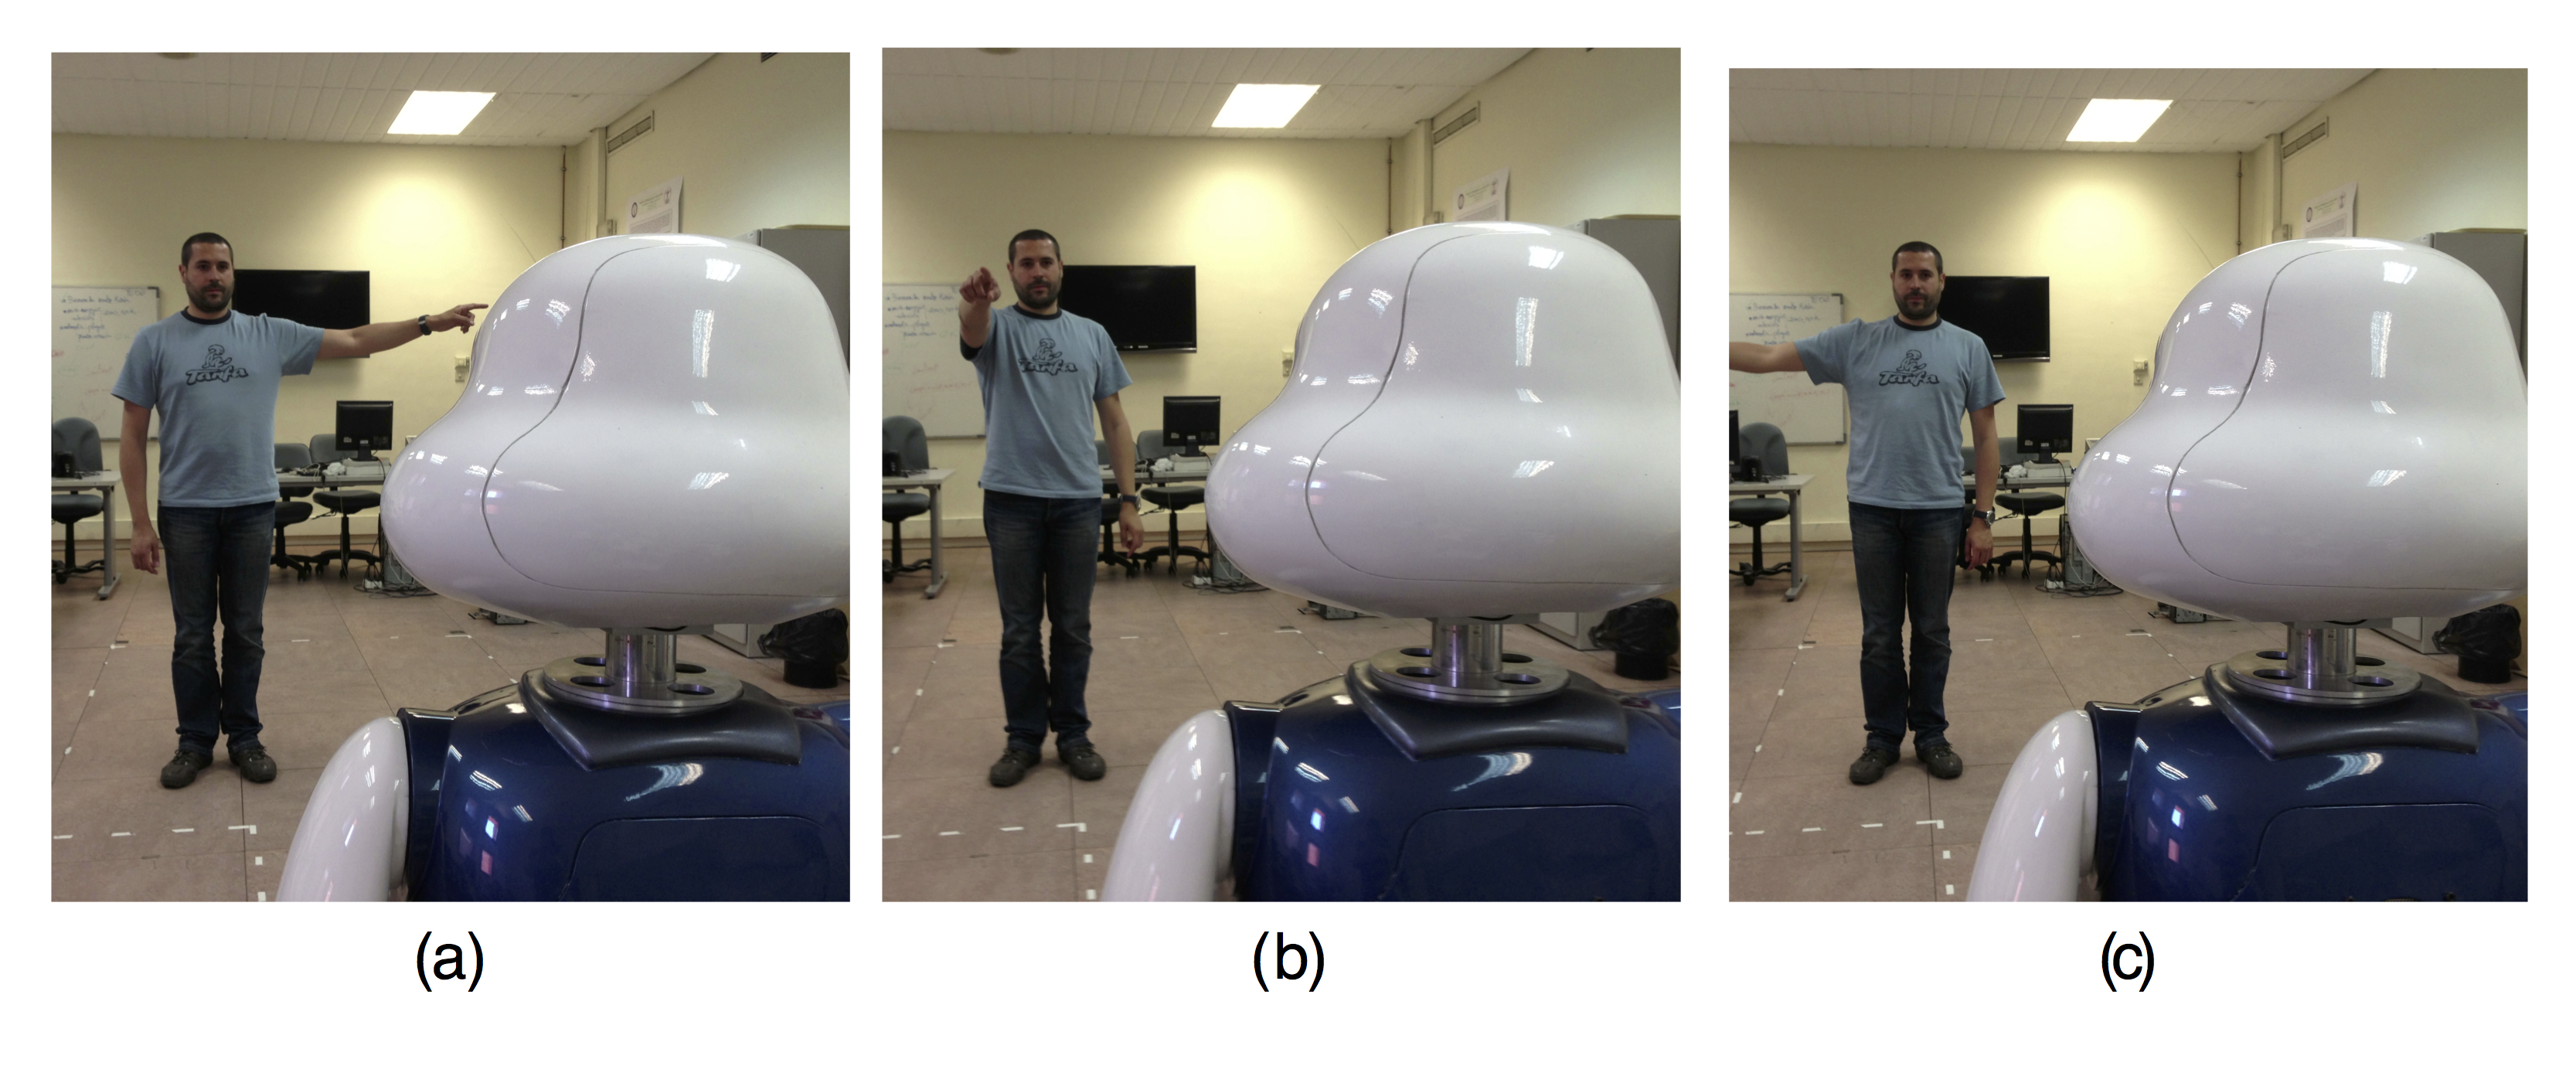
\includegraphics[width=13cm]{Figures/Set3}
\centering
\caption{Photo example of a user pointing. Retrieved \cite{Gonzalez-Pacheco2013}. \label{fig:set3}}
\end{figure}

The users were free to point in the way they preferred. This led to a variety of combinations of arms and positions for the same pose. In Figure \ref{fig:poses} shows examples of users pointing. The color gray represents users posing forward, color blue represents users pointing left, and color green represents users pointing right. 

\begin{figure}[h]
\includegraphics[width=8.5cm]{Figures/Poses}
\centering
\caption[Examples of how different users pointed during the training for pointing poses.]{Examples of how different users pointed during the training for pointing poses. Gray represents users posing forward, blue represents users pointing left, and green represents users pointing right.  Retrieved form \cite{Gonzalez-Pacheco2013}. \label{fig:poses}}
\end{figure}

Each direction at which the users were pointing was labelled as a learning class: \emph{pointing right}, \emph{pointing left} and \emph{pointing forward}. Within each class, there are different subclasses depending on the combinations of arms. In the tables in Appendix A all the combinations and the users that present them are exposed.

The experiment consists in showing the system these examples one by one. The system is able to detect if they belong to different classes by itself, and it learns those new classes when detected. 

However, first we had to understand the problem by observing the data we were dealing with. The work in this Thesis, consisted in initially analyzing these datasets for the purpose of applying novelty detection on them, and then performing such experiments. 

The first question presented is if this data is linearly separable. Using Principal Component Analysis \footnote{PCA is a "statistical procedure that uses an orthogonal transformation to convert a set of observations of possibly correlated variables into a set of values of linearly uncorrelated variables called principal components" \cite{pca}}, all the examples were reduced to 2 dimensions and plotted, as can be seen in Figure \ref{fig:exp03}. Red dots represent users pointing \emph{right}, green dots represent users pointing \emph{forward} and blue dots represent users pointing \emph{left}. The datasets are not linearly separable in 2D.

\begin{figure}[h]
\includegraphics[width=14cm]{Figures/exp03}
\centering
\caption{2D reduction for the pointing dataset with original data. \label{fig:exp03}}
\end{figure}

Observing the different skeletons, we could see that the position of the legs was also very diverse. Because of the location of the Kinect camera, from a low position with respect to the torso and looking upwards, the legs in some users could not be recorded properly. This provoked that some of the entries of the dataset do not have legs at all of the legs appear distorted. Using a One-Class SVM outlier detection, we could confirm that the outliers detected furthest form the frontier were those with legs not recorded properly. Also, the center of the torso of the users was not always recorded at the position (0,0,0), as can be seen in Figure \ref{fig:origin_poses}. The frame of reference used was the Kinect's. For that reason, if different users did not locate at the exact same spot, the x,y,z location of their joints would differ.

\begin{figure}[h]
\includegraphics[width=4.5cm]{Figures/origin_poses}
\centering
\caption[Original data referenced to the Kinect's frame of reference]{Original data referenced to the Kinect's frame of reference. The users moved when recording the poses, so each skeleton was located in a different point. The novelty detection system is more sensible to the differences in the skeleton location than to the pose. red: \emph{pointing right}, green \emph{pointing forward} blue: \emph{pointing left}. \label{fig:origin_poses}}
\end{figure}

Since we are interested in finding differences in the data, this led to the data being very different because of the legs or because of the reference of the torso. Those are not the differences we are interested in, we want the data to be different because it represents pointing each of the three poses. Thus, we need all of the poses to have the same frame of reference. To accomplish this, the torso was moved to the point (0,0,0) and  all the other joints were normalized with respect to the torso. Figure \ref{fig:origin_poses_mod} shows the skeletons shape after the normalization.

\begin{figure}[h]
\includegraphics[width=4.5cm]{Figures/origin_poses_mod}
\centering
\caption[Original data with torso referenced to (0,0,0)]{Original data with torso referenced to (0,0,0). Now all the skeleton's joints are normalized with respect to the torso, located in the origin. red: \emph{pointing right}, green \emph{pointing forward} blue: \emph{pointing left}. \label{fig:origin_poses_mod}}
\end{figure}

The parts of the body that are pore representative of the pointing pose are mostly the arms and the torso, since the users titled their shoulders to point. Thus, we decided to get rid of the legs and hips data points for each user, removing 9 joints: right and left foot, right and left knee and right and left hip. Figure \label{fig:pca} shows the PCA reduction after the modification of the data.

\begin{figure}[h]
\includegraphics[width=14cm]{Figures/exp03_centered}
\centering
\caption{2D reduction for the pointing dataset with modified data. \label{fig:pca}}
\end{figure}

We still cannot separate each of the 3 types of poses linearly. The areas of interest, where the problems may appear, are those where two or more poses merge. 

The final dataset used for the experiments has the following parameters:

\begin{description}
\item[Size]: 87 instances \\ 29 users, 3 instances each, \emph{pointing right}, \emph{pointing forward} and  \emph{pointing left}
\item[Dimensionality]: 81 parameters \\ 9 remaining joints with 8 attributes each $ji = (x,y,z,qx,qy,qz,qw,C)$
\end{description}

\section{Method} \label{4.3}

The data with the poses was provided in .arff files \cite{arff}. Each file consisted of the set of skeletons produced by one user in a session of the experiment mentioned in Section \ref{4.1}. The number of entries of data was different for each user, and it depended on the time that user was recorded. The average number of entries for each user was 218, with a standard deviation of 182. 

The data shape of the data was described in equations \ref{eq-4.1}, \ref{eq-4.2} and \ref{eq-4.3}.

Each entry was formed by $t$ the time stamp, $u$ the user ID, $J$ the set of 15 joints, with 8 attributes each, and $L$ the label of the entry, being \emph{stand pointing right}, \emph{stand pointing left} and \emph{stand pointing forward}. The total number of columns was 124.

A preprocessing step was carried out. It consisted in cleaning the irrelevant columns. These include the label, user-id, h-stamp and all columns corresponding to the position of feet, knees, and hips. The final entries had 81 columns. The data is divided by user and by pose. Each entry represents an user pointing in one of the three directions.

The  novelty detection system uses four algorithms, GMM, One class SVM and K-means, from the Scikit-Learn Machine Learning Library \cite{scikit-learn}, and  Least Squares Anomaly Detection (LSA), that was developed by Jonh Quinn \cite{lsa}. LSA implementation file can be found in his webpage. 

The experiments were carried out with Python \cite{python} programming in a IPython notebook \cite{ipython}. All the experimental data and scripts that were written for this thesis are public and can be accessed in \cite{github}. The IPython notebook was also published in nbviewer \cite{notebook}.The representation of the data was done using the python library Matplotlib\cite{matplotlib}. Other python libraries used for the treatment of the data were Pandas\cite{pandas} and Numpy\cite{numpy}.

\section{Experimental setup}

The system had to be tested with different experiments to demonstrate the accomplishment of the different objectives fo the Thesis. 

1. Firstly, we had to test that the system is able to filter noise. This means that it has to recognize a new pose as \emph{interesting} when it has seen similar poses happen frequently before it, and ignore the entry when it is detected as \emph{noise}. We tested what was the frequency that made the poses become interesting.

2. Secondly, we had to test the performance of the different algorithms to recognize strange entries in the data. The performance was measured training the system with entries only from one pose, e.g. \emph{pointing right}, and testing the system with entries from the same pose and from the other two poses. The entries from the same pose should be detected as \emph{known} and the entries from other poses should be detected as \emph{strange}

\subsection{Algorithms used} \label{4.4.1}

The algorithms used for the experiments are One class SVM, LSA, K-means and GMM.

\textbf{One class SVM and LSA} algorithms provide directly a label that classifies the entries as anomalous or normal. We have translated this labels to the numerical system (1, 0). An entry is assigned a novelty score of 1 when it is detected as anomalous, and a novelty score 0 when it is detected as normal. In the noise filter, a novelty score of 1 is obtained for noisy entries, and a 0 for interesting entries. In the strangeness evaluation test, a 1 is achieved for strange entries, and a 0 for known data. 

\begin{table}[h]
    \begin{tabular}{ c c c c}
    \hline
    Label from the algorithm & Novelty score for the entry $x$ & Noise filter & Strangeness test \\ 
    \hline
    anomalous & 1 & noise & strange \\
    normal & 0 & interesting & known \\
    \hline
    \end{tabular}
    \centering
    \caption[One Class SVM and LSA label interpretation]{One Class SVM and LSA label, for and extry $x$, translation to the binary system. The meaning of the binary novelty scores in the noise filter corresponds to the third column. The fourth column represents the outcome of the binary novelty scores in the strangeness test.}
\end{table}  


\textbf{K-means and GMM} provide a fitting score, the corresponding novelty score calculation from the fitting score was explained in Sections \ref{3.1} and \ref{3.2}. When the novelty score for an entry is lower than 1, the entry is classified as normal and when it is higher than 1 it is classified as anomalous. As mentioned in Section \ref{3.3}, these novelty scores can be tuned depending on the sensitivity desired, with the \emph{curiosity factor}. In the noise filter, a novelty score higher than 1 is obtained for noisy entries, and lower than 1 for interesting entries. In the strangeness evaluation test, a higher than one score is achieved for strange entries, and lower than 1 for known data.

\begin{table}[h]
    \begin{tabular}{ c c c}
    \hline
    Novelty score for the entry $x$ & Noise filter & Strangeness test \\ 
    \hline
    novelty.score(x) $\geq$ 1 & noise & strange \\
    novelty.score(x) $<$ 1 & interesting & known \\
    \hline
    \end{tabular}
    \centering
    \caption[K-means and GMM novelty score interpretation]{K-means and GMM novelty score interpretation for and entry $x$ to the interestingness and strangeness tests. The meaning of novelty score in the noise filter corresponds to the third column. The fourth column represents the outcome of novelty score in the strangeness test.}
\end{table}

An entry that is classified as both \emph{interesting} and \emph{strange}, is considered a \emph{novelty}.

\subsection{Graphic Interface}

A graphic interface was created to show the results of the tests and the shape of the skeletons we were considering, it can be seen in Figure \ref{fig:graphic}.

\begin{figure}[h]
\includegraphics[width=15cm]{Figures/results_imp/right_vs_left1}
\includegraphics[width=15cm]{Figures/results_imp/right_vs_left2}
\includegraphics[width=15cm]{Figures/results_imp/right_vs_left3}
\centering
\caption[Graphic interface]{Graphic interface for the experiments showing, in the right side, the interestingness test of new \emph{pointing left} entries with a base of knowledge of \emph{pointing right} entries. \label{fig:graphic}}
\end{figure}

In the Figure \ref{fig:graphic} we can see the interestingness tests on the left side, the 3D plot corresponds with the representation of the 3D data of the skeletons, and the bar plot representing the noise scores computed for the entry in black. The higher the noise score, the less interesting the entry is to the system. While the noise score is higher than or equal to 1, the entry analyzed is seen as noise, and we do not want to know anything else from it. The bars in this case will be painted red for a visual alert. However, if the noise score is lower than 1, that means that the entry is interesting, and the system wants to pay attention to it, the bars for in this case will be green. 

On the right side, the strangeness test is presented. Once the new entry has passed the noise filter, and thus has been detected as interesting, the system wants to find out if it is part of a known class, or if it is a strange class it has never seen before. If the strangeness score is higher than or equal than 1, the entry is predicted as strange, and thus, as it was interesting and now is algo strange, we can say that it is a novelty, according to its definition in the \textbf{Definitions} section. With this result, the bars are colored green, since the system detected what is the objetive of this Thesis, a novelty. If the strangeness score is less than 1, it means that the entry is a known entry, entries like it are already known by the system, and the bars are colored red. Table \ref{tab:color} summarizes all these cases. 

The Figure \ref{fig:graphic} shows how in each row we showed a new \emph{pointing left} entry to the system. All of the entries added to the system accumulate to calculate the noise score of the new entry, as explained in Section \ref{3.2}. The two first rows show that the entries ponting left are considered noise, as the noise score is higher than 1. However, when we add the third \emph{pointing left} entry, the noise scores lower and are now lower than 1, the system has found that \emph{pointing left} happen frequently, and that it should pay attention to them. Then, it allows the strangeness test to take part. This follows the general scheme we designed in Chapter \ref{Chapter3} and can be seen in Figure \ref{fig:int}. 

\begin{table}[h]
    \begin{tabular}{ c c c c c}
    \hline
    Noise score & Color bar noise & Strangeness score & Color bar strange. & Entry pred. \\ 
    \hline
    $\geq$ 1 & red & - & - & noise\\
    $<$ 1 & green & $<$ 1 & red & known\\
    $<$ 1 & green & $\geq$ 1 & green & novelty\\
    \hline
    \end{tabular}
    \centering
    \caption[Color code for the interface]{ Color code for the interface depending on the noise score and the strangeness score of an entry. \label{tab:color}}
\end{table}

\section{Results}

\subsection{Part 1. Noise filtering by interestingness evaluation}

Figure \ref{fig:graphic} shows how the test for detecting interesting entries is showed to the user. We are interested in knowing what is the frequency of appearance that a pose needs to stop being noise and start being detected as interesting. In other words, how many times do the user needs to pose in front of the system in the same way, for the system to detect that the user is doing something that it needs to pay attention to.

In the example in Figure \ref{fig:graphic}, a base of knowledge of \emph{pointing right} entries was taught to the system. We are testing how many entries of \emph{pointing left} we had to show to the system so it realizes that they are not noise anymore. We are trying to figure out when a new entry of \emph{pointing left} will be considered interesting. As a reminder, by doing this the system is filtering noise entries that may enter to the system once and never be repeated. 

\begin{figure}[h]
\includegraphics[width=11cm]{Figures/Esquema_interest}
\centering
\caption{Interest evaluation step located in the general scheme. \label{fig:int}}
\end{figure}

As the system has not learned any \emph{pointing left} entries yet, the strangeness test in the right side shows that the strangeness acore is higher than 1, thus the entry is strange. As the entry has been classified as interesting and strange, it is considered a novelty, this process can be seen in \ref{fig:int}. The strangeness test will be further tested in Subsection \ref{4.5.2}.

Thus, we have shown that, actually, the system needs a frequency of appearance of a new pose to pass the noise filter.  In the case of Figure \ref{fig:graphic}, the frequency needed to detect the pose as interesting is 2. The third time a pose is showed to the system, it is considered interesting.

The following plot, in Figure \ref{fig:chart}, shows the general performance for the interestingness evaluation.  The plot shows the evolution of the noise score for the different algorithms. The X axis represents how many users with the same pose have been showed to the system. The Y axis represents the averaged noise score from the algorithms, extracted from 63 try-outs. A point below the noise threshold line, corresponding to the value 1, means that the entry is detected as not noise, and thus it is interesting. We consider that, at least, for the first user with a new pose showed to the system, the system should detect it as noise and not pay attention to it, so the score should be higher than 1 in the first X point.

\begin{figure}[h]
\includegraphics[width=14cm]{Figures/results_imp/Chart}
\centering
\caption[Noise score evolution when adding from 1 to 5 users of an unknown class to the system]{Noise score evolution when adding from 1 to 5 users of an unknown class to the system. Comparison of the different algorithms. Points below the threshold line indicate that the user is considered interesting. \label{fig:chart} }
\end{figure}

We can see that both GMM and K-means consider the new pose as noise when it has been showed only once and twice to the system. When it is showed a third time, the algorithms detect that it is now interesting, so it will pass to the next phase detecting whether should be added to the normal dataset or not. The noise scores obtained for the different algorithms was averaged from 63 tests, with different pose combinations. Figure \ref{fig:chart} plots the mean and standard deviation from these results, and Table \ref{tab:int} shows their numerical values. 

As can be seen in Table \ref{tab:int}. One class SVM  also shows a significant decrease in the score when the third user is showed. The mean of the scores for the first user is 0.89. This indicates that, in a 11$\%$ of the cases, the first user showed to the system was detected as interesting already, as thus, the noise filter with One Class SVM filter failed. LSA does not show a very good performance with this analysis, in Table \ref{tab:int}, we can see that the average detection for the first user is 0.38, meaning that the noise filter misses 62$\%$ of the cases when the new pose is presented the first time. 

\begin{table}[!ht]
	\footnotesize
	\renewcommand{\arraystretch}{2}
	\begin{tabular}{cccccc}
	\hline 
	 & 1 user    &  2 users &  3 users & 4 users    &  5 users \\
	\hline
	GMM  & 4.36$\pm$0.7  & 1.42$\pm$0.3 & 0.35$\pm$0.07 & 0.15$\pm$0.02 & 0.006$\pm$0.01\\
	K-means  & 5.1$\pm$1.2 & 1.42$\pm$0.25 & 0.56$\pm$0.10 & 0.38$\pm$0.06 & 0.32$\pm$0.06    \\
	One class SVM  & 0.89$\pm$0.07 & 0.77$\pm$0.10 & 0.28$\pm$0.10 & 0.33$\pm$$\pm$0.11 & 0.39$\pm$0.12  \\
	LSA   & 0.38$\pm$0.01 & 0.11$\pm$0.07 & 0.0$\pm$0.0& 0.0$\pm$0.0& 0.0$\pm$0.0   \\
	\hline
	\end{tabular}
	\centering
	\caption[Data corresponding to the graph in Figure \ref{fig:chart}]{Data corresponding to the plot in Figure \ref{fig:chart}. It resumes the average noise scores and the standard deviation for each algorithm. Represents the noise score evolution when showing from 1 to 5 users of an unknown class to the system. Comparison of the different algorithms. $ K_{GMM} $ = 3, $ K_{Kmeans} $=1. \label{tab:int}}
\end{table}

$ K_{GMM} $ and $ K_{Kmeans} $ represent the \emph{curiosity factors} for each algorithm, they were chosen as a example for this Experiment. Since we can modify the sensitivity of GMM and K-means, changing the curiosity factor presented in Section \ref{3.4}, we could also modify the frequency needed for the entries to be considered interesting. Instead of being 2, as in this case,  we could increase it of decrease it. For this purpose, the curiosity factor should be calculated empirically for each application, and is out of the scope of the work in this Thesis. As we have explained in the Subection \ref{4.4.1}, One Class SVM and LSA do not have curiosity factors since they provide a label directly.

From the point of view of our analysis, the algorithms that perform best to detect the interestingness of a new entry are GMM and K-means.

\subsection{Part 2. Strangeness evaluation} \label{4.5.2}

The second step for the system, after a new data was detected as interesting, was finding out if that data was already known by our system or it was a novelty, novelty i.e. our model could not predict it. Here we present the results of testing the performance of the different algorithms to recognize strange entries in the data. This step can be located in the general scheme in Figure \ref{fig:stran}. 

\begin{figure}[h]
\includegraphics[width=11cm]{Figures/Esquema_strange}
\centering
\caption{Interest evaluation step located in the general scheme. \label{fig:stran}}
\end{figure}

\subsection{Global novelties}

Global novelties are those detected between poses, we want to differentiate \emph{pointing right} from \emph{pointing left} or \emph{pointing forward}. To evalute the performance of the different algorithms for this task, different experiments were carried out with the existing dataset.

\subsubsection{Size of the base of knowledge}

The dataset was separated by poses, \emph{stand pointing right}, \emph{stand pointing left} and \emph{stand pointing forward}. Each user has an entry for each pose. 

\begin{description}
\item[Size]: 87 instances \\ 29 users, 3 instances each, \emph{pointing right}, \emph{pointing forward} and  \emph{pointing left}
\item[Dimensionality]: 81 parameters \\ 9 remaining joints with 8 attributes each $ji = (x,y,z,qx,qy,qz,qw,C)$
\end{description}

The system was tested for each of the three poses. The experiment consisted on teaching the system one of the poses, creating a model with different sizes of base of knowledge of that pose, with 5, 10 and 20 users respectively. Then, the system had to classify 5 entries of each of the other 2 poses, and 10 entries of that same pose, as seen in Table \ref{Tglo2}. The expected result is that all the entries from different poses will be detected as novel, and all the entries from the same pose will be detected as known.

\begin{table}[h]
    \begin{tabular}{cc}
    \hline
    Training (normal) & Testing (normal + novel) \\ 
    \hline
    5 & 10+10 \\
    10 & 10+10 \\
    20 & 10+10 \\
    \hline 
    \end{tabular}
    \centering
    \caption{Benchmark of the dataset size for the experiments in size of the base of knowledge. \label{Tglo2}}
\end{table}

The parameters used to measure the performance were given in terms of Binary classification. The binary classification calculates different parameters in terms of test outcomes for the entries. If the test is positive (1) the entry is classified as an novelty, if it is negative (0) it is classified as known.

Imagine we get a new data $y_1$. We know that $y_1$ is really a novelty, so $y_1 = 1$. Knowing this, we test it with the system and retrieve an novelty classification prediction. The prediction is labeled as $y_1'$.

If our system predices: 
\begin{equation}
\begin{split}
y_1' = 1 \mbox{, we obtain a True Positive (TP)} \\
y_1' = 0\mbox{, we obtain a False Negative (FN)}
\end{split}
\end{equation}

Now we get a new data, that we know it's not novel, $y_2 = 0$, and test it with the system. The prediction of the system is now labeled as $y_2'$.

\begin{equation}
\begin{split}
y_2' = 0\mbox{, we obtain a True Negative (TN)} \\
y_2' = 1\mbox{, we obtain a False Positive (FP)} 
\end{split}
\end{equation}

The following metric, the F score, was used to evaluate the performance of the algorithms:

\begin{equation}
F score = \dfrac{2 \times TP}{2 \times TP+FN+FP}
\end{equation}

Following, we present a set of results that assess how the size of the base of knowledge affects the F score performance of the algorithms. The experiment was repeated 30 times, 10 for each pointing pose, and the results were averaged. Table \ref{size} present the results for each size.

\begin{table}[!ht]
	\footnotesize
	\renewcommand{\arraystretch}{2}
	\begin{tabular}{p{1.2cm}p{0.7cm}p{0.6cm}p{0.7cm}p{0.7cm}p{0.6cm}p{0.7cm}p{0.7cm}p{0.6cm}p{0.7cm}p{0.7cm}p{0.6cm}p{0.7cm}}
	\hline 
	 & \multicolumn{3}{c}{GMM}& \multicolumn{3}{c}{One class SVM}& \multicolumn{3}{c}{LSA}& \multicolumn{3}{c}{K-means} \\
	Size  & Mean    & SD & SE& Mean    & SD & SE& Mean    & SD & SE& Mean    & SD & SE \\
	\hline
	5  & 0.73 & 0.05 & 0.04 & 0.73 & 0.10 & 0.07 & 0.28 & 0.21 & 0.15 & 0.62 & 0.18 & 0.13 \\
	10 & 0.81 & 0.07 & 0.05 & 0.74 & 0.11 & 0.08 & 0.53 & 0.26 & 0.18 & 0.55 & 0.19 & 0.13 \\
	20 (a)  & 0.00 & 0.00 & 0.00 & 0.78 & 0.10 & 0.07 & 0.58 & 0.24 & 0.17 & 0.41 & 0.27 & 0.19    \\ 
	20 (b) & 0.84 & 0.06 & 0.05 & 0.78 & 0.10 & 0.07 & 0.58 & 0.25 & 0.17 & 0.42 & 0.27 & 0.19    \\
	\hline
	\end{tabular}
	\centering
	\caption[Novelty detection F score performance with different sizes of knowledge]{Novelty detection F1 parameter performance of the different algorithms when detecting a new entry  with different sizes of the base of knowledge. All trials: $ K_{Kmeans} $ = 1. (5) $ K_{GMM} $ = 30, (10) $ K_{GMM} $ = 3, (20(a)) $ K_{GMM} $ = 3, (20(b)) $ K_{GMM} $ = 0.1  Note: Size = number of users in the base of knowledge, SD = Standard Deviation, SE = Standard Error \label{size}}
\end{table}

We can observe that the F score performance of GMM, One class SVM and LSA all increase with the expansion of the base of knowledge, they perform better the bigger the base of knowledge is. On the other hand, K-means performs better the smaller the base of knowledge is. This relies on the mathematical methods used by the different algorithms. This behavior from K-means was unexpected, and we will need to look further into it in future iterations of the system.  

The $ K_{GMM} $ has to be modified depending on the size of the base of knowledge. In 20(a), we can see that without the modifying $ K_{GMM} $, all the entries are detected as normal. Thus, $ K_{GMM} $ needs to be decreased, to make the system more sensible. In the trial with 5 users, $ K_{GMM} $ needs to be increased to 30, since none of the entries were detected as normal with a $ K_{GMM} $ of 3, thus the system is less sensible. The $ K_{Kmeans} $, on the other hand, was suitable for all fo the trials. This relies on the calculation of the algorithm score provided by the Scikit Learn API. This results show how to the $curiosity$ $factors$ can be choosen empirically. We found that $ K_{GMM} $=3 did not work for a base of knowledge of 20 users, and we had to increase it, however,  $ K_{Kmeans} $ did not need to be changed. As this question is out of the scope of this Thesis, no further trials were carried out, and the $curiosity$ $factors$ used in this experiments will be the ones used in the rest of the experiments, each one corresponding with the appropiate size of the base of knowledge.

\begin{table}[h]
    \begin{tabular}{cc}
    \hline
    Size of the base of knowledge & $ K_{GMM} $ \\ 
    \hline
    5 & 30 \\
    10 & 3 \\
    20 & 0.1 \\
    \hline 
    \end{tabular}
    \centering
    \caption{$ K_{GMM} $ used for the different sizes of the base of knowledge}
\end{table} 

\subsubsection{Comparison of the performance for the different set of poses}

To analyze more in detail the performance of the algorithms for global novelty detection, we realized a more thorough analysis, performing the tests on \emph{stand pointing right}, \emph{stand pointing left} and \emph{stand pointing forward} separately. 

The system was tested for each of the three poses. This time, the experiment consisted on teaching the system one of the poses, training a model with \textbf{10 random users} of that pose. Again, the system had to classify 5 entries of each of the other 2 poses, and 10 entries of that same pose, , as explained in Table \ref{Tglo}. The expected result is that all the entries from different poses will be detected as novel, and all the entries from the same pose will be detected as known.

\begin{table}[h]
    \begin{tabular}{cc}
    \hline
    Training (normal) & Testing (normal + novel) \\ 
    \hline
    10 & 10+10 \\
    \hline 
    \end{tabular}
    \centering
    \caption{Benchmark of the dataset size for all of the experiments in global novelties. \label{Tglo}}
\end{table}

This test was carried out 10 times per pose. Tables \ref{global} show the results obtained for the different poses. The first row in the table corresponds with a base of knowledge of \emph{pointing right}, the second with \emph{pointing left} and the third with \emph{pointing forward}.

Table \ref{global} summarizes the F score performance of the algorithms for the different poses.

\begin{table}[!ht]
	\footnotesize
	\renewcommand{\arraystretch}{2}
	\begin{tabular}{p{1.2cm}p{0.7cm}p{0.6cm}p{0.7cm}p{0.7cm}p{0.6cm}p{0.7cm}p{0.7cm}p{0.6cm}p{0.7cm}p{0.7cm}p{0.6cm}p{0.7cm}}
	\hline 
	 & \multicolumn{3}{c}{GMM}& \multicolumn{3}{c}{One class SVM}& \multicolumn{3}{c}{LSA}& \multicolumn{3}{c}{K-means} \\
	 & Mean    & SD & SE& Mean    & SD & SE& Mean    & SD & SE& Mean    & SD & SE \\
	\hline
	RIGHT   & 0.87 & 0.07 & 0.02 & 0.87 & 0.06 & 0.02 & 0.87 & 0.05 & 0.02 & 0.81 & 0.08 & 0.03    \\ 
	LEFT  & 0.80 & 0.04 & 0.01 & 0.72 & 0.09 & 0.03 & 0.24 & 0.21 & 0.07 & 0.24 & 0.10 & 0.03  \\
	FORWA.  & 0.90 & 0.04 & 0.01 & 0.78 & 0.12 & 0.04 & 0.50 & 0.17 & 0.06 & 0.20 & 0.26 & 0.09 \\
	\textbf{Average} & \textbf{0.86} & 0.04 & 0.03 & \textbf{0.79} & 0.06 & 0.04 & \textbf{0.54} & 0.26 & 0.18 & \textbf{0.42} & 0.28 & 0.20 \\
	\hline
	\end{tabular}
	\centering
	\caption[Novelty Detection F score performance for global novelties]{Novelty Detection performance for global novelties. Novelty Detection F score performance of the different algorithms when detecting a new entry with a base of knowledge of \emph{pointing right} entries in the first row, \emph{pointing left} in the second and \emph{pointing forward} in the third. $ K_{GMM} $ = 3, $ K_{Kmeans} $=1. Note: SD = Standard Deviation, SE = Standard Error \label{global}}
\end{table}

As a general overview of the results presented in this table, we can say that GMM overperforms all other three algorithms in each of the poses and in average.

for \emph{pointing right}, in the first row of Table \ref{global}, the F score performance of all algorithms is similar. Achieving a 87$\%$ of F score for GMM, LSA and One Class SVM, and a 80$\%$ for K-means. For this concrete pose, we cannot highlight a concrete algorithm, since each one has its own pros and cons. In Appendix A, \ref{metrics}, the results  are expanded with more metrics, showing the precision, recall and accuracy.   

for \emph{pointing left}, in the second row of Table \ref{global}, the F score performance of all algorithms lowers with respect to \emph{pointing right}, this is specially critical for LSA and K-means. It is important to take into account that \emph{pointing left} has many variants within the class, as it can be seen in Appendix A. This may lead to have sub classes that differ a lot from each other, like \emph{pointing left} with the right hand or with the left hand. This problem is addressed in subsection \ref{in}, when detecting in-class novelties.

\emph{Pointing forward}, in the third row of Table \ref{global}, led to the best F score performance with GMM. On the contrary, the worst F score was achieved with K-means, and LSA obtained a very poor performance. \emph{pointing forward} also contains in-class variants that may affect to the result achieved, and will be studied in subsection \ref{in}. 

\subsection{In-class novelties} \label{in}

We found a worse performance of the algorithms when trained with the classes \emph{pointing left} and \emph{pointing forward}, so we decided to test this classes more specifically. In-class novelties are defined as novelties within a class. We divided the poses of this classes in sub-classes. The aim is to test if the system would detect if the user is pointing left with his/her right arm or with his/her left arm. The sub-classifications of the data are displayed in Appendix \ref{AppendixA}. 

The following tests use \textbf{5 users} to train the system, and 6 normal instances and 6 new instances to test the system, as explained in Table \ref{Tin}. The new instances consist of 2 instances belonging to the same class and a different sub class and 4 instances belonging to a different class \footnote{The training instances are fewer than in the tests of Global Novelties because the division in sub-classes did not allow to have a trainig set of 10 instances and 5 instances to test from the same sub class.}. The predicted result is that instances belonging to the same sub class will be detected as normal, and those belonging to a different sub class or a different class will be detected as novel. The sub classes used are described in Table \ref{inclass_d}. 

\begin{table}[h]
    \begin{tabular}{ c c }
    \hline
    Training (normal) & Testing (normal + anomaly) \\\hline
    5 & 6+6 \\
     \hline
    \end{tabular}
    \centering
    \caption{Benchmark of the dataset size for all of the experiments in in-class novelties. \label{Tin}}
\end{table}

\begin{table}[h]
    \begin{tabular}{cc}
    \hline
     & Description \\ 
    \hline
    (a) & \emph{Pointing left}, pointing hand \emph{left} other hand \emph{hanging}   \\
    (b) & \emph{Pointing left}, pointing hand \emph{right} other hand \emph{hanging} \\
    (c) & \emph{Pointing forward}, pointing hand \emph{right} other hand \emph{hanging}  entries \\
    \hline 
    \end{tabular}
    \centering
    \caption{Description of the sets for in-class novelty detection \label{inclass_d}}
\end{table}  

As the size of the base of knowledge, a.k.a. the number of training instances, is smaller than in the previous sub section, we use a different $ K_{GMM} $, which is 30 in this case. Thus, the results cannot be directly compared with all the cases from the previous section. However, we can compare them with the average results from the row corresponding to 5 users in Table \ref{size}, which uses the same $ K_{GMM} $ factor.

Table \label{inclass} summarizes the F score performance of the algorithms for the different poses. In Appendix A, \ref{metrics}, the results obtained are expanded with more metrics, showing the precision, recall and accuracy. 

\begin{table}[!ht]
	\footnotesize
	\renewcommand{\arraystretch}{2}
	\begin{tabular}{p{1.2cm}p{0.7cm}p{0.6cm}p{0.7cm}p{0.7cm}p{0.6cm}p{0.7cm}p{0.7cm}p{0.6cm}p{0.7cm}p{0.7cm}p{0.6cm}p{0.7cm}}
	\hline 
	 & \multicolumn{3}{c}{GMM}& \multicolumn{3}{c}{One class SVM}& \multicolumn{3}{c}{LSA}& \multicolumn{3}{c}{K-means} \\
	 & Mean    & SD & SE& Mean    & SD & SE& Mean    & SD & SE& Mean    & SD & SE \\
	\hline
	(a)  & 0.92 & 0.07 & 0.02 & 0.77 & 0.08 & 0.03 & 0.95 & 0.07 & 0.02 & 0.84 & 0.09 & 0.03       \\
	(b)   & 0.73 & 0.08 & 0.03 & 0.72 & 0.07 & 0.02 & 0.32 & 0.20 & 0.07 & 0.62 & 0.16 & 0.05    \\
	(c)  & 0.71 & 0.13 & 0.04 & 0.69 & 0.10 & 0.03 & 0.58 & 0.23 & 0.08 & 0.54 & 0.22 & 0.07    \\
	Average   & \textbf{0.79} & 0.09 & 0.07 & \textbf{0.73} & 0.03 & 0.02 & \textbf{0.58} & 0.31 & 0.22 & \textbf{0.67} & 0.13 & 0.09   \\
	\hline
	\end{tabular}
	\centering
	\caption[Novelty Detection F score performance for in-class novelties]{Novelty Detection performance for in-class novelties. Novelty Detection F score performance of the different algorithms when detecting a new entry with a base of knowledge of (a)\emph{Pointing left}, pointing hand \emph{left} other hand \emph{hanging}, (b) \emph{Pointing left}, pointing hand \emph{right} other hand \emph{hanging} (c) \emph{Pointing forward}, pointing hand \emph{right} other hand \emph{hanging}  entries. $ K_{GMM} $ = 30, $ K_{Kmeans} $=1. Note: SD = Standard Deviation, SE = Standard Error \label{inclass}}
\end{table}

Again, GMM outperformed the other three algorithms in average. However, we can observe an important increase in the performance of K-means, while the average performance of One-Class decreased.

The row corresponding to (a) in Table \ref{inclass} shows that the performance for the in-class novelty detection increases significantly, specially for LSA and Kmeans. The F score for LSA goes from a 24 $\%$ to a 95 $\%$ and for K-means from a  24 $\%$ to a 84 $\%$. In GMM and One Class SVM we can also see an increase, but not so significant. This results show that, in fact, in class novelties are relevant and affect the performance of the system. 

The rows (b) and (c) in Table \ref{inclass}, we prove that this is not an isolated event. In (b) the system is trained with another sub class withing the \emph{pointing left} class, and the performance also increases with respect to the general \emph{pointing left} performance presented in the previous Section.


This also applies to in-class novelties within the \emph{pointing forward} class, as row (c) in Table \ref{inclass}. The F score for LSA goes from a 50$\%$ to a58 $\%$ and for K-means from a  20$\%$ to a 54$\%$. In One Class SVM we can also see an increase, but not so significant. However, the GMM algorithm still outperforms the other three and its performance is lower than when the system was trained with entire classes in Table \ref{global}.


\subsection{Novelties in multi-class systems}

As one of the objectives in the Thesis if that the system learns continuously, at some point the system may have learned \emph{pointing right} and \emph{pointing forward} and the new entry corresponds to a new class \emph{pointing left}. Figure \ref{fig:two} shows the graphic interface for this experiment. The following tests show the performance of the system when faced with this problem of knowing two classes and being asked to classify a third.

\begin{figure}[h]
\includegraphics[width=15cm]{Figures/results_two/two_classes}
\centering
\caption[Graphic interface for multi-class systems]{Graphic interface showing, in the right side, the interestingness test of new \emph{pointing left} entries with a base of knowledge of \emph{pointing right} and \emph{pointing forward} entries.\label{fig:two}}
\end{figure}

\begin{table}[!ht]
	\footnotesize
	\renewcommand{\arraystretch}{2}
	\begin{tabular}{p{1.2cm}p{0.7cm}p{0.6cm}p{0.7cm}p{0.7cm}p{0.6cm}p{0.7cm}p{0.7cm}p{0.6cm}p{0.7cm}p{0.7cm}p{0.6cm}p{0.7cm}}
	\hline 
	 & \multicolumn{3}{c}{GMM}& \multicolumn{3}{c}{One class SVM}& \multicolumn{3}{c}{LSA}& \multicolumn{3}{c}{K-means} \\
	New class  & Mean & SD & SE& Mean & SD & SE& Mean & SD & SE& Mean & SD & SE \\
	\hline
	RIGHT  & 0.67 & 0.19 & 0.10 & 0.79 & 0.07 & 0.03 & 0.70 & 0.18 & 0.09 & 0.84 & 0.06 & 0.03      \\
	LEFT  & 0.68 & 0.02 & 0.01 & 0.82 & 0.03 & 0.02 & 0.60 & 0.05 & 0.03 & 0.69 & 0.13 & 0.06    \\
	FORWA.  & 0.78 & 0.07 & 0.03 & 0.74 & 0.10 & 0.05 & 0.53 & 0.17 & 0.09 & 0.67 & 0.05 & 0.03    \\
	Average & \textbf{0.71} & 0.05 & 0.04 & \textbf{0.78} & 0.03 & 0.02 & \textbf{0.71} & 0.10 & 0.07 & \textbf{0.73} & 0.08 & 0.05  \\ 
	\hline
	\end{tabular}
	\centering
	\caption[Novelty Detection F score performance for multi-class novelty detection]{F1 parameter performance of the different algorithms when detecting a new entry of the 'New class' with a base of knowledge of the other two classes. $ K_{Kmeans} $ = 1 $ K_{GMM} $ = 0.8  Note: New class = new class presented to the system, SD = Standard Deviation, SE = Standard Error}
\end{table}

The best average performance corresponds with One Class SVM this time. The results will be discussed in the Discussion section \ref{discussion}


\section{Discussion} \label{discussion}

The presented results show that it is possible to build a system that distinguishes when new poses are interesting and strange. And thus, the system does not pay attention when unusual poses happen once, but it becomes curious when an unusual pose happens several times, and it can't recognize it. 

We have shown that our current systems does not detect an entry as interesting until similar entries have appeared twice before. This filters out noisy entries that may appear, and the system will not bother the user by asking too many times. As seen in the performance graph in Figure \ref{fig:chart}, the algorithms that work best from our approach are GMM and K-means.

For GMM, One class SVM and LSA, the performance increased when we increased the size of the base of knowledge, meaning that we trained the system with more instances of the normal pose. However, the performance of K-means lowered. Thus, for future applications, when we start the learning process and we only have access to a small number of training instances, K-means would perform better. But as the systems learns and increases the size the base of knowledge, we may want to switch and use one of the other three algorithms.

The results also show that the $ K_{GMM} $ had to be modified depending on the size of the base of knowledge. $ K_{GMM} $ needs to be decreased as the size of the base of knowledge increases, to make the system more sensible to strange classes. This conforms with the preconceived idea we had. The more the system has seen, the more probable it is that new entries will seem somehow similar to what it knows, and the more sensible it has to be to detect novel entries.

The results also show that the system is able to distinguish between known data and novel data for global and in class novelties. Nevertheless, we have seen that the performance of the system depends highly on the pose we train the system with. The worst performance was achieved when we trained the system with random users from the \emph{pointing left} class. We later saw that the \emph{pointing left} class could be divided in sub classes, and the performance of some of the algorithms increased greatly when the system was trained with this sub classes separately. In average, the best performance results for both global novelties and in-class novelties was achieved by GMM.

We also saw that it is possible to learn continuously and keep operating. This means to train the algorithm with two poses and detect a third one as novel. This is called multi-class novelty detection. However, the performance of GMM lowered in this test, with One Class SVM achieving the best result. The performance achieved by K-means was the best with respect to the other two experiments. We think we cannot extact general conclusions for multi-class novelty detection, since we only tried sets of a maximum of two normal classes. However, this is a good indication for the idea of building in the future a multi-class novelty detection that is able to learn more than 3 classes.

We must stress that this was not a trivial problem to work with. The datasets used, as displayed in Appendix A, included many variations within the poses, and some of them were very similar without belonging to the same class, see \emph{pointing forward} with the right hand and \emph{pointing left} with the right hand. The differences for most of the users was very slight. 

To conclude, we can see these results as a proof of concept. They show that it is possible to build a continuous learning framework, where the robot actively seeks for new examples and asks questions to its teacher about the concepts being learned. This Thesis has not dealt with asking questions about the data, since that would be more specific to an application. But our system knows \emph{when} to ask questions about it. It opens the door to future applications in different fields, and this method and system can be extrapolated to other learning problems inside or outside pose recognition. It is specially relevant in Human-Machine interaction, since our system breaks down the steps of the curiosity process in human behavior.   


%----------------------------------------------------------------------------------------